%Use Lualatex for interpretation!
% lualatex -interaction=nonstopmode --shell-escape DeveloperDocumentation.tex

%You have to have those fonts in your system:
% - Calibri (standard windows font)
% - Trebuchet MS (standard windows font)
% - GROTESKIA (http://www.dafont.com/groteskia.font)

\documentclass[12pt,a4paper]{report}

\newcommand*{\DEVDOC}

%\usepackage[utf8]{inputenc} % for old latex interpreters
%\usepackage[english]{babel}

\usepackage{polyglossia}
\setdefaultlanguage[variant=american]{english} % or ?british
\setotherlanguage{czech}

\usepackage{url}
\usepackage{geometry}
\usepackage[cmyk]{xcolor}
\usepackage{amsmath}
\usepackage[some]{background}
\usepackage{listings}
\usepackage[stable]{footmisc}
\usepackage{titlesec}
\usepackage{fontspec}
\usepackage{epstopdf,epsfig} 

\usepackage{xr-hyper}

\definecolor{TextanDarkRed}{cmyk}{.37,.94,.83,.59}
\definecolor{TextanRed}{cmyk}{.0,.879,.844,.220}
\definecolor{javagreen}{rgb}{0.25,0.5,0.35}

\newfontfamily\chapterfont{GROTESKIA}
\newfontfamily\sectionfont{Trebuchet MS}

\titleformat{\chapter}{\chapterfont\fontsize{36pt}{1pt}\selectfont\color{TextanRed}}
  {\thechapter}{20pt}{\chapterfont\fontsize{36pt}{1pt}\selectfont\MakeUppercase}
\titlespacing{\chapter}{0pt}{0pt}{20pt}
\titleformat*{\section}{\LARGE\sectionfont\color{TextanDarkRed}}
\titleformat*{\subsection}{\fontsize{14pt}{1pt}\selectfont\sectionfont\itshape\color{TextanDarkRed}}
%\titleformat*{\subsubsection}{\sectionfont\color{TextanDarkRed}}

\setmainfont{Calibri}

\backgroundsetup{
scale=1,
angle=0,
opacity=1,
contents={
\begin{tikzpicture}[remember picture,overlay]
  \path [fill=TextanDarkRed] (-0.5\paperwidth,-0.5\paperheight)rectangle (-0.37\paperwidth,0.5\paperheight);
 \end{tikzpicture}}
}

\usepackage[unicode,colorlinks=true]{hyperref}
\hypersetup{pdftitle=TextAn - user documentation}
\hypersetup{pdfauthor={Petr Fanta, Duc Tam Hoang, Adam Huječek, Václav Pernička, Jakub Vlček}}
\hypersetup{linkcolor=black, citecolor=black, urlcolor=black, filecolor=black}

\def\chapwithtoc#1{
\chapter*{#1}
\addcontentsline{toc}{chapter}{#1}
}

% sets numbering for subsubsection
\setcounter{secnumdepth}{3}
\setcounter{tocdepth}{3}

\lstdefinelanguage{properties}{% new language for listings
  basicstyle=\ttfamily,
  sensitive=false,
  morecomment=[l]{\#},      % comment
  morestring=[b]",          % string def
  commentstyle=\color{javagreen},
  basicstyle=\small
}

%Comment macro
%Usage:
% \comment[_assignee_]{_author_}{_comment_}
% \comment{_author_}{_comment_}
\makeatletter
\newcommand{\comment}[3][\@empty]{
  {\color{magenta}[#3 - }
  {\color{green}\ifx\@empty#1\relax Author: #2 \else Assignee: #1; Author: #2\fi}{\color{magenta}]}
}
\makeatother

\newcommand{\textan}{\emph{Text\-An}}

\externaldocument[USR-]{../UserDocumentation/UserDocumentation}[../UserDocumentation/UserDocumentation.pdf]


\begin{document}

\begin{titlepage}
\BgThispage
\newgeometry{left=4.5cm,top=7cm,bottom=3cm}

\begin{figure}
 
\includegraphics{../Logos/TEXTAN_logo_grey_B}
\end{figure}
\noindent
\textcolor{TextanRed}{\chapterfont\fontsize{48pt}{1pt}\selectfont\MakeUppercase{Developer documentation}}\\[15pt]
\textcolor{TextanDarkRed}{\sectionfont\LARGE\MakeUppercase{Version 0.1}}

\vfill
\noindent
\begin{minipage}[b]{.75\textwidth}
\textbf{Authors}\\
Petr Fanta\\
Duc Tam Hoang\\
Adam Huječek\\
Václav Pernička\\
Jakub Vlček
\end{minipage}% This must go next to `\end{minipage}`
\begin{minipage}[b]{.25\textwidth}
\textbf{Supervisor} \\
Ondřej Bojar\\
%\vfill
\\
\\
\textbf{Date}\\
\today
\end{minipage}

\end{titlepage}
\restoregeometry

\pagenumbering{roman}
\tableofcontents

%\setlength{\parskip}{1em}
%\chapter*{Intro}
%\addcontentsline{toc}{chapter}{Intro}


\chapter{Introduction}
\pagenumbering{arabic}

\section{Introduction to the project}
Status: A dummy documentation - Text Analyser

Generally, the Police often generate documents with regards to a specific person (criminal records, conflict, ...). 
In the documents, there is a lot of information such as
person's name, their location, date of birth, name of other persons, other persons' location, etc.
There is a need for an application to manage such documents in a convenient way and extract the important details without much human effort.
This is the topic of our software project, called Text Analyser (TextAn).

TextAn is a client-server application for analysing text.
It is intended to manage documents and exploit the information contained in them.
Given a collection of written texts (typically police reports) in Czech language,
TextAn automatically breaks down the unstructured text to exploit the structured information. 

Furthermore, the application allows users to add/remove/adjust the structured information.
They can change the relations, correct mistakes or provide further information.
The structured information could be displayed in graph-view,
\comment[Tam]{Adam, Ondrej}{profile? What is this about?}
which is a fancy way that users could look at his/her profile. 

\comment[anyone]{Adam}{add footnote linking chapter with used libraries when ready}
TextAn is implemented in Java 1.8 using Spring Framework, Hibernate database layer and other libraries.
\comment[Venca]{Adam}{is this correct?}
The data can be stored within any SQL-like relation database, e.g. MySQL.

The developer team consists of 5 students:

\begin{itemize}
\itemsep0em
\item Petr Fanta
\item Duc Tam Hoang
\item Adam Huječek
\item Václav Pernička
\item Jakub Vlček
\end{itemize}

\comment[Petr]{Tam}{please assemble two of my introductions}
Status: An even dummer introduction - Text Analyser

TextAn (Text Analyser)

Generally, there is a huge amount of unstructured written texts which contain structure information.
It ranges from newspapers, medical bills to even personal letters.
In every written document, there are entities like names, address, dates, etc.
These entities do not stand alone, there are relationships between them.
The relationships could facilitate the problem of assigning an entity from new text to an existing objects already stored in the system.
Such problem of extracting structure information out of general documents has recently gained attention from both research and industry.

Czech Police reports are typical example of unstructured sources which contain structured information.
They are the descriptions with regard to a specific person, their profile and actions, criminal records and so on.
Such information is by no doubt the most valuable data in the whole document.
Currently, the extracting is done manually.
In other words, there is a person who reads through all documents,
looks at the database and match the description in the document with the existing data.
This is not-surprisingly very time-consuming and labour-intensive. 

Project TextAn is devoted to build a pleasant and effective tool for extracting structured data in Czech police reports. 
Our goal is to provide an effective extraction of structured data with user involvement.
It consists of three main contributions.
\comment[Venca]{Adam}{is it efficient? :-D}
First, an efficient design of database for structured data is implemented.
Second, we aim to maximize the performance of automatic detection of entities.
\comment{Tam}{This may be wrong. Think how to make it clear}
\comment{Adam}{Seems ok to me.}
Third, TextAn is designed to provide a friendly method for users to confirm or adjust the system's suggestions.
At first, the second task may achieve lown recognition accuracy,
but with the semi-automatic approach the user input together with the magic of machine learning could improve the performance significantly. 


%\section{Conventions}

\section{Glossary}
\comment{Petr}{Copy glossary form User documentation, or remove the reference into
Client usage.}

Terms are used in very specific manner in the documentation and in both the
client and the server, therefore it is really essential to understand their
meaning. Otherwise, it is possible to misunderstand the rest of the text.

\comment[anyone]{Petr}{check if this makes sense!}
\begin{description}
\item[Document]
The document is an arbitrary text that is processed by \textan{}. E.g. a police
report, a letter, a movie review or a judgment. In the following text the terms
document and report are used interchangeably.

\item[Object]
The term "object" refers to our representation of some unique thing in
\textan{}. Consider for example a person with name Joseph Smith from Prague with
identifier 000123/4567. The object refers to this person in the real world, in
meat and bones.

\item[Alias]
The alias represents a designation of a object. For example: Joseph Smith, Joe
Smith, Joey S., J. Smith or just Smith can be names of one concrete person.
Names are aliases for the person.

\item[Entity]
An entity is a sequence of words recognized either by a named entity recognizer
or by a user. \comment[Petr]{Petr}{Move to next paragraph - Object assigment}
The entity will be later assigned to an object and it becomes an alias
of the object. Consider for example the sentence: Joe Smith was seen
in Prague on 5th September. The sentence contains 3 entities: Joe Smith (person),
Prague (city), 5th September (date). We don't know which objects belong to these
entities yet. Prague can represent the capital city of the Czech Republic,
or a city in the USA.

\item[Object/Entity Type]
Each object and each entity has a type. For example person, date, city, country
etc. The set of types in the system depends on the domain which the system is
deployed to.

\item[Object Assigment]
\comment[Petr]{Petr}{Description of object assigment}

\item[Alias occurrence]
\comment[Petr]{Petr}{Description of alias occurence}

\item[Object Merging]
\comment[Petr]{Petr}{Description of object merging}

\item[Relation]
The relation represents any relationship between objects mentioned in a document.
A relation can be represented in a document by an anchor word, or it can be
unexpressed, which means without any anchor in a document. See Anchor below.
\comment[anyone]{Adam}{Check this sentence with two relations, one with anchor, one without anchor.}
Consider this example: "Adam (890524/1367) is married to Eve". Three objects
appear in the sentence - persons Adam and Eve and the id 890524/1367. There
are two relations: Adam "has" 890524/1367 without an anchor and Adam "marriage"
Eve with the anchor "married".

\item[Relation Type]
Each relation has a type. For example born, reside, die, kill etc. Similarly to
object/relation types the set of relation types in the system depends on the
domain which the system is deployed to.

\item[Anchor]
An anchor is a word or a sequence of words that is bound to a relation between
objects. Consider for example the sentence: Joey Smith killed Mary-Ann S. There
is a relation between Joey Smith and Mary-Ann S., which is represented by the
word "killed". The word is the anchor. \comment{Ondrej}{Why do you not write
about type here?}

\item[Roles and orders]
Each object in a relation can have a role assigned. This role is mostly used
for visualisation and storing additional information. Moreover object can also
have order assigned which is just an integral number used for graph
visualization\ifdefined\USRDOC{} (see Section \ref{sssec:EditRelations})\fi{}
\ifdefined\DEVDOC{} (see Section \ref{USR-sssec:EditRelations} in the user
documentation)\fi{}. For example relation created from sentence
"Bill killed Joe." could be represented like this:
Bill (-1, murderer) --kill--> (1, victim) Joe.
\end{description}



\chapter{Requirements specification}
\comment{Petr}{If we need to make the documentation longer, include the whole specification}
% Chapter: Requirements spec.

\section{Functional requirements}
\subsection{Mandatory functional requirements}
This section contains a list of functional must be implemented in the final solution.

\begin{itemize}
	\item The system recognizes entities in a document and determines their type.
	\item The system assigns recognized entities to objects from the database.
	\item An user will be able to edit recognized entities (add an entity, remove
	an entity, change a type of of an entity, change a range of an entity).
	\item An user will be able to edit assignments of objects to entities.
	\item An user will be able to mark relations between objects.
	\item An user will be able to add types of entities (respectively objects)
	and relations.
	\item The system will continuously learn to recognize entities and to assign
	objects to entities from processed documents confirmed by an user.
	\item An user will be able to merge objects saved in the database.
	\item An user will be able to browse objects and relations between them stored
	in the database as lists and as graphs.
	\item An user will be able to use to browse the database these kinds of search:
	\begin{itemize}
		\item a full text search in documents,
		\item a searching of objects or relations by types,
		\item a searching of objects by their aliases,
		\item and combinations of these methods.
	\end{itemize}
	\item An user will be able to suspend work on a currently processed document.
	\item Ongoing changes will be stored locally, they will be stored in the database
	collectively after completion work on the document.
	\item The database must log (revise) all performed changes.
\end{itemize}

\subsection{Optional functional requirements}
\comment{Petr}{Add some explanation. Or not?}
\begin{itemize}
	\item An user will be able to cancel a merging of objects followed by
	a semi-automatic assignment of object occurrences, that was recognized while
	they were merged, to divided objects.
	\item The system will recognize relations between objects in a document by
	relations that an user marked before in other documents.
	\begin{itemize}
		\item An user will be able to edit recognized relations between objects
		in a document.
	\end{itemize}
	\item An user will be able to use to browse the database more complex kinds
	of search:
	\begin{itemize}
		\item a search of connection between objects,
		\item a search of relations by anchors in documents.
	\end{itemize}
\end{itemize}

\section{Non-functional requirements}
\begin{itemize}
	\item The system must support a parallel connection of more users.
	\item The system must be able to recover from a crash of server or client.
	\item The system must be connectible with other systems.
	\item The system must reasonably handle a unavailability of server.
	\item An updating of auto-recognition, a learning from new examples,  may take
	a longer time, the system should use an old model during the learning.
	\item The system must be usable without an Internet connection, e.g. in
	a closed intranet.
\end{itemize}

\section{Fixed limits} \comment{Petr}{Is it correct name for this section?}
\begin{itemize}
	\item Entities are contiguous and not overlap in a document.
	\item An user won't be able to edit a data stored in a database. The only form
	of update will be insertion of a new document and its annotations.
	\item A parallel annotation of a document won't be supported.
	\item The system won't solve an authentization and  an authorization of users.
	\item The system won't solve a backup.
\end{itemize}




\comment{Petr}{where to place use cases, mockup screens etc?}

\comment{Adam}{I will place use case, mockups etc. here for now...}

\comment{Adam}{It could be interesting if the sequence diagram is extended to include server components too.}
\comment{Petr}{Maybe only for some communication, definitely not all}

\begin{figure}[!htb]
        \centering
        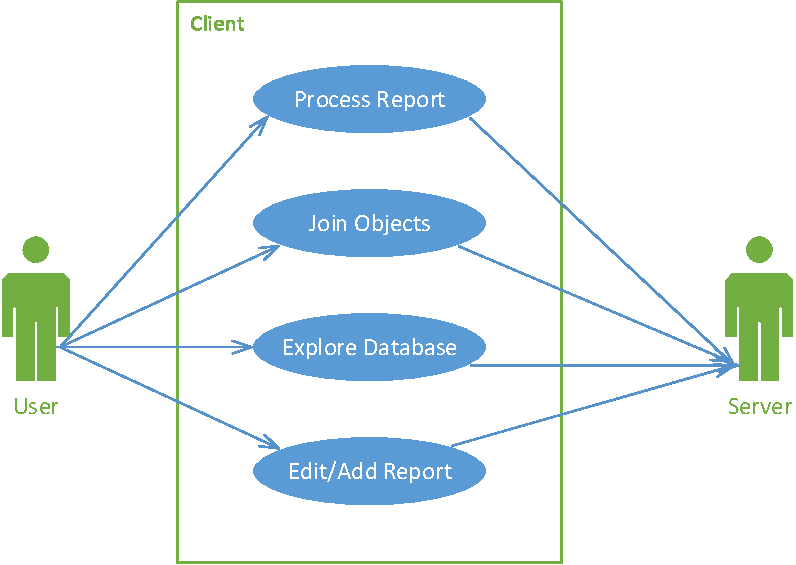
\includegraphics[width=\textwidth]{Images/UseCase1}
        \caption{Use case of the end-user.}
        \label{fig:UseCase1}
\end{figure}

\begin{figure}[!htb]
        \centering
        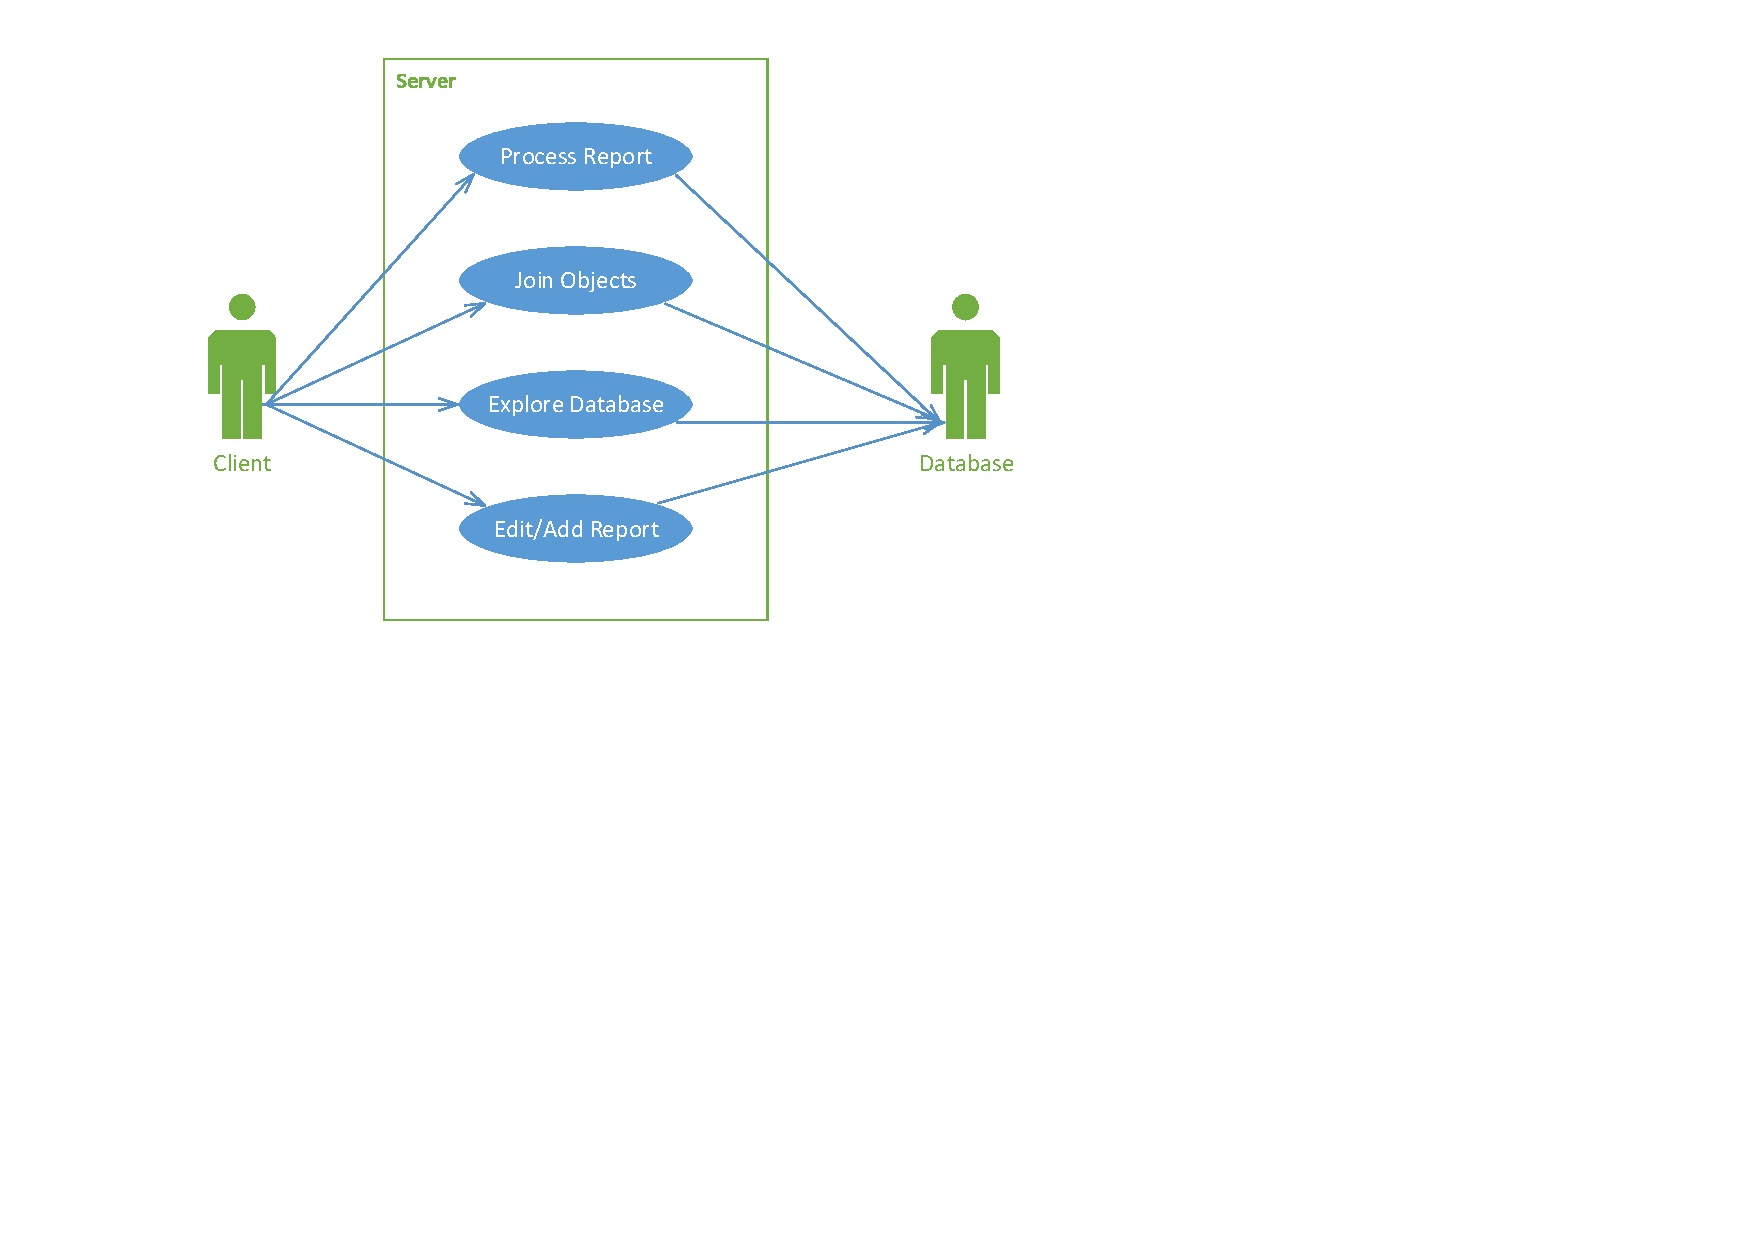
\includegraphics[width=\textwidth]{Images/UseCase2}
        \caption{Use case of the client.}
        \label{fig:UseCase2}
\end{figure}

\chapter{Analysis}

\section{Related work}
%This section provides details on other projects/publications which are in the similar fields.

Mining structured information from unstructured text documents has recently gained attention.
Current approaches are still far from an fully automated and completely accurate processing.
However, the challenge has led to a number of research and applications.
Each work focused on solving a particular problem in the big pictures with regard to some specific languages. 

This section provides an insight into other contributions to the mining problem.
Both research-oriented works and industry applications are taken into account.

\subsection{Knowtator}
% http://knowtator.sourceforge.net/
% http://knowtator.sourceforge.net/docs/Ogren_HLT-NAACL06_Demo_Abstract_Final.pdf
Knowtator is a general-purpose text annotation tool.
Developed by scientists at Division of Biomedical Informatics, 
it uses Protégé knowledge-base as the database.
As an early development of tool for annotating data, Knowtator has a number of limitations (OS dependent, no client-server, no automatic detection).
The remarkable feature of Knowtator is the ability to relate annotations to each other via the slot \textit{reference}.
The tool has been implemented as a Protégé plug-in for wider-spread usage.

\subsection{Anafora}
%http://www.aclweb.org/anthology/N/N13/N13-3004.pdf
%Anafora: A Web-based General Purpose Annotation Tool

Anafora is an open source web-based text annotation tool,
developed by scientists of University of Colorado at Boulder.
It distinguishes itself from previous contribution in the field of OS platform.
Before the introduction of Anafora, old tools were written as a local application in a local machine under the threat of data fragmentation.
Anafora is a web-based tool with client-server structure. % OK, INTRODUCTION TO ANAFORA

\begin{figure}[!htb]
	\centering
	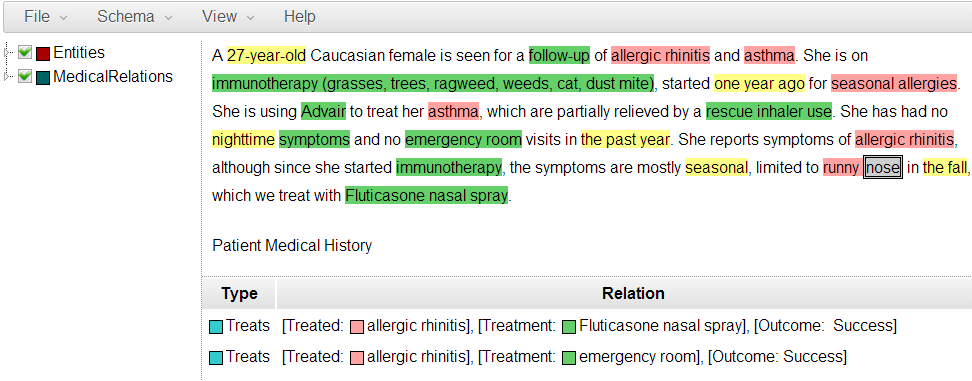
\includegraphics[width=\textwidth]{Images/anafora}
	\caption{Anafora graphics user interface}
	\label{fig:First}
\end{figure}

Anafora is designed for the medical domain with a medical named entity tags, not a general domain.
It is developed with a server in Django (a Python framework) and a client in jQuery (a JavaScript library).
Besides, it stores annotations in each single XML files.
By doing so, authors claim that the tool is agile and flexible.
The project hierachy is designed to be the file/directory structures.
The application provides an automatic detection of named entities.
Users can change/add details to the annotation by mouse or keyboard.
Anafora was designed for English.

The limitation of Anafora lies in the data structure.
Complicated definitions like relations (or relation properties) among entities
are not supported. It may be the trade-off when authors want to develop lightweight
tools based on a data structure such as XML.

\subsection{BRAT}
% http://brat.nlplab.org/

BRAT rapid annotation tool is a web-based tool for text annotation,
most useful to add notes to existing text documents (taken from the introduction of BRAT).
It is developed by the University of Tokio.
This tool does support the linking relation between two entities and even the link from entities to a definition outside documents (such as Wikipedia).

\begin{figure}[!htb]
	\centering
	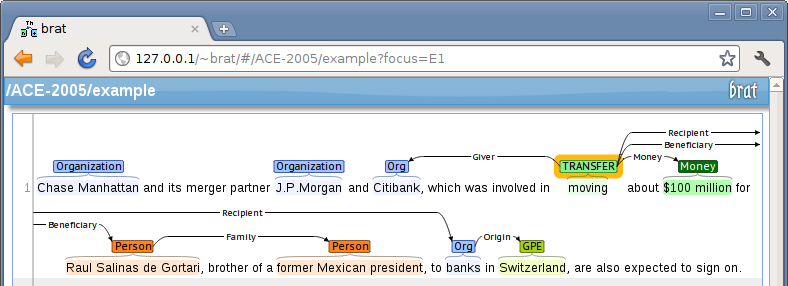
\includegraphics[width=\textwidth]{Images/brat}
	\caption{BRAT graphics user interface}
	\label{fig:Second}
\end{figure}

The strong point of BRAT is the simplicity of usage.
The tool offers a comprehensive visualization with mouse-based activities,
a method for linking to an external resources (such as Freebase, Wikipedia, and Open Biomedical Ontologies).
A number of other useful functions are \textit{save, export from standoff format, search}.
The brat \comment{Ondrej}{BRAT?} standoff format is a simple format developed for the visualization of the tool,
in which data is stored in two files: a text file \textit{.txt} and an annotation file \textit{.ann}.

The weak point of the tool is that it does not support any automatic recognition of entities.
All annotations have to be done manually.
This leads to a feature that the tool could be applied on a wide range of languages.
However, the limitation leads to a fact that BRAT is merely an editor for annotating.


\section{Adopted solutions and decisions}
\comment{Ondrej}{Is this right name? Shouldn't be adopted solutions and decisions placed after specification?}
%%%%%%%%%%%%%%%%%%%%%%%%%%%%%%%%%%%%%%%%%%%%%%%%%%%%%%%%%%%%%%%%%%%%%%%%%%%%%%%

\subsection{Used Technologies}

This section lists all technologies and libraries used in \textan.

%TODO are links to the libraries missing intentionally? Adam
\paragraph{Apache CXF}
Apache CXF is an open-source Web services framework. CXF implements the JAX-WS 
standard APIs, is configurable through Spring and can be embedded into Jetty,
Tomcat or other servlet containers.

\paragraph{ControlsFX}
ControlsFX is a Java8 open source library aiming at enhancing the programming
experience with standard JavaFX. It provides wide selection of new and improved
components to make everyday use of JavaFX even easier. \textan\ uses it mainly for
its high quality and user-friendly standard dialogs which are incomprehensibly
and sorely missing in JavaFX.

\paragraph{Hibernate ORM}
%TODO Venca
Hibernate ORM (Hibernate in short) is an object-relational mapping library for
the Java language, providing a framework for mapping an object-oriented domain
model to a traditional relational database. Hibernate solves object-relational
impedance mismatch problems by replacing direct persistence-related database
accesses with high-level object handling functions.

\paragraph{Hibernate Search}
Hibernate Search is a library (or Hibernate ORM extension), which integrates
the full text library functionality from Apache Lucene in the Hibernate and
JPA model. It offers full-text search support for objects stored by Hibernate
ORM, Infinispan and other sources. Think of it as Google\texttrademark\ for
entities: search words with text, order results by relevance and find by
approximation (fuzzy search).

\paragraph{Java-ML}
%TODO Kuba/Tam
Java-ML is a machine learning library for Java. It is a collection of machine
learning and data mining algorithms.

\paragraph{Jetty}
Jetty is a pure Java-based HTTP (Web) server and Java Servlet container. It can
be embedded into other applications through Jetty API.

\paragraph{JUNG}
JUNG (Java Universal Network/Graph Framework) is older Java library for
displaying graphs, still widely used in Java world, well documented and easily
extensible. Sadly, it does not support JavaFX, but only older Java GUI framework
SWING. Fortunately, thanks to new JavaFX8 SwingNode enabling usage of SWING
components in JavaFX scenes it was possible to seaminglessly integrate JUNG into
JavaFX \textan\ Client.

\paragraph{JFXtras}
JFXtras is another JavaFX8 enhancing project. \textan\ Client uses it mostly for
its window management capabilities enabling extensible use of inner windows
embedded into the main window. Another used component is BigDecimalField which
brings common Spinner component into JavaFX.

\paragraph{MorphoDiTa}
Morphological Dictionary and Tagger is an open-source tool for morphological
analysis of natural language texts. It performs morphological analysis, 
morphological generation, tagging and tokenization and is distributed as
a standalone tool or a library, along with trained linguistic models. In
the Czech language, MorphoDiTa achieves state-of-the-art results with 
a throughput around 10-200K words per second. MorphoDiTa is a free software
under LGPL license and the linguistic models are free for non-commercial use
and distributed under CC BY-NC-SA license, although for some models the original
data used to create the model may impose additional licensing conditions.

\paragraph{NameTag}
NameTag is an open-source tool for named entity recognition (NER). NameTag 
identifies proper names in text and classifies them into predefined categories,
such as names of persons, locations, organizations, etc. NameTag is distributed
as a standalone tool or a library, along with trained linguistic models.
In the Czech language, NameTag achieves state-of-the-art performance
(Straková et al. 2013). NameTag is a free software under LGPL license and the 
linguistic models are free for non-commercial use and distributed under CC 
BY-NC-SA license, although for some models the original data used to create
the model may impose additional licensing conditions.

\paragraph{PretopoLib}
Although JUNG is mature and well thought library, it lacks one important feature
out-of-the-box: displaying hypergraphs. For this reason JUNG graph rendering
part of PretopoLib is used. PretopoLib is a library mainly focusing on
pretopology and graph displaying is rather byproduct. However it fully meets our
requirements and its author kindly provided us the sources so we could fix one
inconvenient detail.

\paragraph{SLF4J \& Logback}
Simple Logging Facade for Java (SLF4J) provides a Java logging API by means
of a simple facade pattern. The underlying logging backend is determined
at runtime by adding the desired binding to the classpath and may be
java.util.logging, log4j or logback.

\paragraph{Spring Framework}
The Spring Framework is an open source application framework and inversion
of control container for the Java platform. The framework's core features
can be used by any Java application, but there are extensions for building
web applications on top of the Java EE platform.


\chapter{Architecture}
% Chapter: contains the system architecture

%For every one: use as many diagrams as possible :) (author Petr)

The architecture of \textan{} is based on client-server model. Two main components
are the \textan{} server and \textan{} client which communicate via W3C web services
(SOAP protocol).



\comment{Ondrej}{Mention why it was split like this - a wish from outside, but in 
the future fully automated (tuned) annotation without client}

\comment{Petr}{This explanation should be rather in \ref{sec:Decisions}}



\section{Communication}
\label{sec:Communication}
\comment[Petr (\& Adam)]{Petr}{Describe communication pattern between client and server,
sequence diagram etc.}

The communication between the client and the server is stateless, because the processing
of a document by a human user may take a very long time, especially because of the saving
of documents during processing in the client. Sessions cannot be used on
the server side, because they can die due to timeout before end of the processing.
For this reason, the state of a processing is placed on client side and is transferred
with each request in situations where it is necessary.

Usage of webservice \emph{DataProvider} is straightforward, its operations are
completely independent and are intended for viewing and manipulating
the database.

The service \emph{DocumentProcessor} is more demanding and needs its operations
called in specific order to achieve proper recognition (see Figure
\ref{fig:ClientServerCommunication}). First of all, the client needs to obtain
the ticket which stores information about processing and is needed for all
following calls. For three recognition operations there are two variants. First
for processing report already stored in the database (called\emph{*ById}) and
second for inserting completely new document to the database (called
\emph{*FromString}). Operations \emph{getEntities*} recognize entities in
given report. Operations \emph{getAssignments*} assign objects from the database
to recognized entities and finally operations \emph{getRelations*} recognize
relations between objects. Please note that \emph{getRelations*} is not
implemented in this version of \textan{} and returns empty response with no
relations.

The recognition operations do not store anything into the database. For this
purpose there are three operations \emph{saveProcessedDocumentFromString} and
\emph{saveProcessedDocumentById} with similar differences as mentioned above.
The third operation \emph{rewriteAndSaveProcessedDocumentById} has as input
parameters both document id and document text, because it overwrites the report
text stored in the database. It is intended to be called when the document has
been changed by others while being processed by the user, so the user can
force returning to the original version or provide new one. All three operations
take \emph{force} parameter specifying whether the saving should happen even
though there have been external changes to the database, e.g. new objects, new
relations and newly joined objects.

If the \emph{force} parameter is \emph{false} and such external changes have
been detected, saving returns \emph{false} and method \emph{getProblems} can be
called to get information about the changes. After making adjustments to
recognizing/assignments if needed, save operations can be called with
\emph{force} parameter set to \emph{true}.

During the processing of a document already stored in the database, other users
can alter it in the database. If this happens, the subsequent call of processing
operation returns fault \emph{documentChangedException} as a warning. If the
user wants to overwrite these changes as mentioned above, the client should
switch to \emph{*FromString} recognizing operations and save the report with
operation \emph{rewriteAndSaveProcessedDocumentById}.

If the document stored in the database has been processed by another user while
being processed by a local user, the subsequent call of processing operation
returns fault \emph{documentAlreadyProcessedException} and the processing must
end as no report can be processed multiple times.

For more details, consult the WSDL descriptions and Javadoc of the server
implementation.


\comment{Adam}{It could be interesting if the sequence diagram is extended to include server components too.}
\comment{Petr}{Maybe only for some communication, definitely not all}

\begin{figure}[!htb]
        \centering
        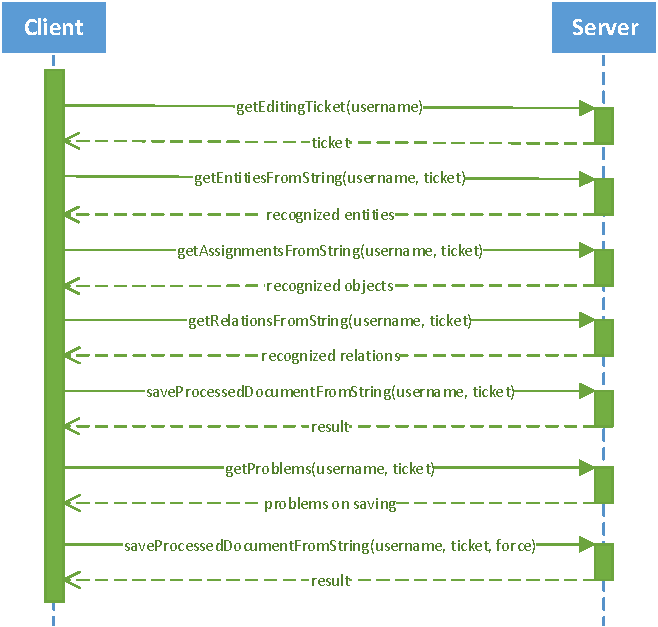
\includegraphics[width=\textwidth]{Images/ClientServerCommunication}
        \caption{Example of Client-Server communication during report processing.}
        \label{fig:ClientServerCommunication}
\end{figure}


\chapter{Developer notes}
\section{Work on the project}
%This section contains work progress
In this section is described work progress in each iteration.

\subsection{Initialization}
\comment[anyone]{Adam}{Add proper rank of Honza}\\
TextAn team visited policeman Jan Hořínek, who introduced us his work and showed
us existing inadequate software whose extension we should prepare. Basis of the
project should be processing police reports - recognize entities and match them
to existing objects in the database. We should use Webservices to provide easy
way to integrate the project to the current system. He promised us models and
example data inputs and expected outputs. We divided the work as follows:

\begin{itemize}
\item \textbf{Petr Fanta} - entities recognition and input parsing, look for useful existing solutions
\item \textbf{Adam Huječek} - GUI validation, component schema and communication
\item \textbf{Václav Pernička} - database
\item \textbf{Peter Šípoš} - web service, graph GUI, testing
\item \textbf{Jakub Vlček} - entities recognition and input parsing, look for useful existing solutions
\end{itemize}

We made some decisions and requirements for each component:

\paragraph{Database}
\comment{Jakub}{attach document schema here?}
At the beginning, we made database schema, which was approved after a few
iterations. We paid attention mainly on schema generality because we want to
support more than one (police) domain.\\
Database should support versioning, parallel processing, partial records. We
decided to create special layer between server and database because of
generality (it will be easier to change database system). Logging (users,
changes) support should not be missing. Problem could be with merging two
objects into new one, so we should create special functionality and table in the
database.

\paragraph{Client}
We decided for pipeline model. This means that report processing will consist of more successive phases:

\begin{enumerate}
\item Report insertion
\item Report editing
\item (Auto) Entity recognition
\item Entity editing (entity types, ranges, creating new ones)
\item (Auto) Object recognition
\item Object editing (adding new ones, repair bad connections between entities and objects)
\item (Auto) Relationships recognition
\item Relationships editing
\item Report confirmed and sent to server
\end{enumerate}

Changes in each phase are not stored in the database immediately but they are
stored locally and write to database follows confirmation. Problem is with
machine recognition, because models with newly added items are trained after final confirmation, so we can't use just machine learning output. We decided, that newly added items will be preferred over recognized ones
 
\subsection{Design \& technologies}
In November, we mainly chose and tested technologies which we could use. Peter
Sipos left \textan{}, but Duc Tam Hoang joined us. His specialization is
linguistic and machine learning so he will be really useful for our project.
Because he is Vietnamese student we had to changed project language to English.
His main task will be NER and entity-object matching. We were trying different
entity recognizers, but there are not many applicable for Czech. Milan Straka
promised us his project NameTag. It is named entity recognizer for Czech, so
exactly what we need. Problem is, that it is not finished yet and in C++
language, so there must be additional layer between Java and C++.
We researched possibilities about entity-object matching. Program will get
entity and assign it possible candidates from objects. This part could not be
purely automatic because of ambiguity, but if there will be high probability,
program should match object entity pair automatically.

Possible solutions for this entity-object matching are machine learning  methods
ranking or classification.

\comment{Petr}{This is not true! In the end we use WEKA, because JavaML project is probably dead.
Also new versions of WEKA are probably more powerful and fits our needs (provide probability from classification) }
We looked for suitable Java library which provides machine learning techniques.
Candidates were JavaML and Weka. After testing these two libraries, we chose
JavaML, because it provides more machine learnig algorithms (some of them uses
Weka library). Weka's problem is that it was created for teaching purposes so
it's performance is not as good as JavaML.

There were two possible server architectures: standalone or embedded webserver
(Tomcat or Jetty). We considered usage of some technologies like Spring, CXF and
Hibernate for database layer.

\subsection{Prototyping \& interconnecting}
After choosing technologies, we made some prototypes of each component. We
discussed a lot APIs (we need them for testing). For testing purposes, we must
provide some mock objects, so everyone implemented mock of his component.
NameTag was released, so we started acquainting with it. After meeting with Milan Straka, where he presented us NameTag, we started becoming more familiar with it and stared testing it.
There were problems with compiling and Java bindings, which took more time than we expected. Problem was missing documentation.
We connected client and database to server, implemented database data browsing on client (mainly graphs viewing with JUNG).
Tam made prototype of object matcher, but it was not integrated to server.

\subsection{Main coding}
When we made a prototype of whole program, everyone started improving his component in his own branch.
\paragraph{Server} Server was debugged and made reliable. It starts using WSDLs so there were lot of work on server and client parts. Result was, that Java code is now generated automatically. Connection to database was reworked to use Spring Beans.
\paragraph{Named entity recognizer} NameTag was fully integrated to server. We started editing it for our purposes (using our structures and types). There were problems with gazetteers files and translating entities from NameTag to Textan.
After receiving information that NameTag will not support JNI to training parts, we researching how to launch training binaries from Java.
\paragraph{Client} Client was reworked to pipeline as we need, we improved graph viewing to support oriented edges.
\paragraph{Object matcher} TextPro (as we called entity-object matching) has first prototype. It uses ranking and than, if ranking has poor result, classification.
\paragraph{Database} Database has new layer with DAOs, so no more need to access database directly.
After this iteration, we released first alpha version of TextAn.

\subsection{Improving}
Alpha version of NameTag learning was implemented. There were few problems with portability because of different architectures and operating systems. After implementation of special functions in database, we made automatic data extraction for learning. For this purpose, new function to server was added - commands. It is implementation of design pattern Command, which started data generation and model training after new report insertion. Models managing implemented due to bigger size (deleting old ones) 
Database support logging. It was done through interceptors - triggers in Hibernate layer.
In client, there were lots of small fixes in GUI, problems were with portability between Windows and Unix-like systems, where ControlsFX and JavaFX behave differently.
TextPro received many new features. We integrated Morphodita because we needed it's tagger for new features.
Settings through properties files are now supported in each component.

\subsection{Bugfixing \& documentation}

\section{Decisions}
\label{sec:Decisions}

\comment{Petr}{Maybe move this section to Analysis}

\chapter{Possibilities of future extensions}
% Chapter: POSSIBILITIES OF FUTURE EXTENSIONS

The chapter introduces some areas, that should be in our opinion extended or
improved. The list does not contain all possible extensions, of course.

\section{Relation Recognition}
The automatic recognition of relations between objects is the most missing
feature in the current version of \textan{}. However, because this task has been
taken into account from the very beginning of the development and because it is
one of the optional requirements, \textan{} contains the whole infrastructure
except for the core component itself.

The recognition can be based on many different criteria, same as relations.
For example: the presence of objects in the same document, the kind of verbs,
which are the anchors for relations in the most cases, their valency and
relations which users marked before in other documents. The component could be
probably based on some machine learning method and above mentioned attributes.

\section{Searching}
Although \textan{} provides several search methods, they are weak compared to
possibilities that graphs offer. Consider for example an environment of police
reports and a task in which you need to find all persons who know a killer. The
graph contains this information, if good model is defined for the domain, but
how can you ask for them?

It implies at least usage of some graph query language and creation of some
graph indexing over the data. Or in better case usage of different data storage. 

\section{Underlaying Database}
In the case that graph operations become more important, it will be better to
use a different data store, for example a NoSql database based on RDF or a graph
database. There are many implementations of these databases, both commercial and
open-source, e.g. OpenLink Virtuoso\footnote{\url{http://virtuoso.openlinksw.com/}},
or Neo4j\footnote{\url{http://www.neo4j.org/}}.

\section{Restrictions for Objects in Relation}
As it is noted in user documentation Section \ref{USR-sec:Domain},
\textan{} is very universal and needs some conventions to provide good results,
because there is no way how to enforce the proper use. The system cannot work
properly without conventions anyway, but some extension enforcing restrictions
can improve overall outcomes.

The most natural improvement is restricting objects in relations. Consider for
example relation type "murder". There must probably be at least one object of
type "person" with role "victim" in the relation of this type, also there
should be an object of type "person" with role "murderer", an object of type
"address" with role "crime place" and so on.

\section{Multiple Languages at Once}
Although \textan{} can be configured for multiple languages, mainly for Czech
and English (see Section \ref{USR-sec:Lang} in the user documentation), it
support only one language at once. It can be useful to support multiple
languages at once. For example, when \textan{} is used by police for analyze
their reports, it can be helpful to manage reports from foreign colleagues in
same system. A similar example is any multinational company and its documents.

This change affects multiple areas in \textan{}, especially recognizers and
the full text indexing and searching, because they use different procedures for
each language and it is difficult to find any universal solution for them. It
means that the system must know which language is currently used and must choose
the right method for processing. It can be solved by multiple models for
recognizers, one for each language, and multiple analyzers for the searching and
the language will have to be defined explicitly.

\section{Client}
The \textan{} client could be improved in many ways as any graphic application.
Some examples:

\begin{itemize}
	\item Filtering in documents could display exact location of matched text
	\item There could be a mechanism to localize object and relation types and
	relation roles
	\item Inner windows could use some layout framework
	\item Inner windows could transform to Outer stages and vice-versa on the
	run
\end{itemize}


\appendix
\chapter{Source codes}

\comment{Petr}{Change appendices from chapter to section?}

\comment{Petr}{Github, DVD}

\chapter{Documentation for Java Sources}
Documentation for Java sources is not a part of this printout, but can be found
in attached DVD in folder Javadoc.

\chapter{Client Properties}
This apendix contains a list of properties from configuration file that controls
client behaviour and their brief description.

\comment[Adam]{Adam}{Add window properties for settings and about windows.}

\begin{lstlisting}[frame=single,language=properties]
#main application window height
application.height=600.0
#is main application window maximized?
application.max=true
#main application window width
application.width=800.0
#main application window x-pos
application.x=192.0
#main application window y-pos
application.y=119.0
#indicator whether the filters in context menus in pipeline
#should be cleared when item is selected
clear.filters=true
#document edit/add window height
document.edit.height=300.0
#is document edit/add window maximized?
document.edit.maximized=true
#document edit/add window width
document.edit.width=450.0
#document edit/add window x-pos
document.edit.x=193.0
#document edit/add window y-pos
document.edit.y=164.0
#document view window height
document.viewer.height=576.0
#is document view window height maximized?
document.viewer.maximized=true
#document view window widht
document.viewer.width=662.0
#document view window x-pos
document.viewer.x=148.0
#document view window y-pos
document.viewer.y=203.0
#number of documents to list on one page in document
#view window
documents.per.page=100
#document list window height
documents.viewer.height=604.0
#is document list window maximized?
documents.viewer.maximized=true
#document list window width
documents.viewer.width=663.0
#document list window x-pos
documents.viewer.x=513.0
#document list window y-pos
documents.viewer.y=87.0
#user wants Object Type with id 1 to be displayed as white
ENTITY.color.1=#FFFFFF
#default distance from graph center to display
graph.distance=6
#graph window height
graph.viewer.height=784.0
#is graph window maximized?
graph.viewer.maximized=true
#flag indicating whether object type filter should be
#displayed in graph viewer
graph.viewer.objectfilter=true
#flag indicating whether relation type filter should be
#displayed in graph viewer
graph.viewer.relationfilter=true
#graph window width
graph.viewer.width=678.0
#graph window x-pos
graph.viewer.x=60.0
#graph window y-pos
graph.viewer.y=26.0
#flag indicating whether the hypergraphs should be displayed
#as background color instead of by additional vertex
hypergraphs=true
#object join window height
join.view.height=682.0
#is object join window maximized?
join.view.maximized=true
#object join window width
join.view.width=953.0
#object join window x-pos
join.view.x=147.0
#object join window y-pos
join.view.y=91.0
#directory lastly used for save/load a report
loadreport.dir=C\:\\temp
#application language
locale.language=cs
#number of documents to list on left page
#in object join window
objects.per.page.left=100
#number of documents to list on right page
#in object join window
objects.per.page.right=100
#number of documents to list on one page
#in object list window
objects.per.page=100
#user wants Relation Type with id 1 to be displayed as white
RELATION.color.1=#FFFFFF
#relation list window height
relation.view.height=741.0
#is relation list window maximized
relation.view.maximized=true
#relation list window width
relation.view.width=722.0
#relation list window x-pos
relation.view.x=149.0
#relation list window y-pos
relation.view.y=15.0
#report wizard pipeline window height
report.wizard.height=734.0
#is report wizard pipeline window maximized?
report.wizard.maximized=true
#report wizard pipeline window width
report.wizard.width=843.0
#report wizard pipeline window x-pos
report.wizard.x=397.0
#report wizard pipeline window y-pos
report.wizard.y=70.0
#report wizard pipeline window height
selectfile.dir=C\:\\temp
#should ssl be used for communication?
ssl=true
#path to trust store
ssl.trustStore=c\:/temp/clientKeyStore
#trust store password
ssl.trustStore.password=MyPass
#trust store type (default JKS)
ssl.trustStore.type=JKS
#files with extension 'txt' should be processed as text files
#encoded in Windows-1250 encoding; only other valid value for
#now is TEXT_UTF8 for utf-8 encoding
selectfile.extension.txt.type=TEXT_CP1250
#url of the data provider wsdl
url.data.wsdl=http\://localhost\:9500/soap/data?wsdl
#url of the data provider
url.data=http\://localhost\:9500/soap/data
#url of the document processor wsdl
url.document.wsdl=http\://localhost\:9500/soap/document?wsdl
#url of the document processor
url.document=http\://localhost\:9500/soap/document
#user's login
username=BFU
#flag indicating whether independent system windows should
#be used instead of embedded inner windows
windows.independent=false
\end{lstlisting}

Dynamic properties \emph{selectfile.extension.X.type} where X is file extension
are used to store information how to extract report from this file type.

Dynamic properties \emph{ENTITY.color.X} where X is Object Type id are used to
store color assigned by user to the given Object Type.

Dynamic properties \emph{RELATION.color.X} where X is Relation Type id are used
to store color assigned by user to the given Relation Type.



\end{document}
